\setcounter{page}{2}
\chapter{Выполнение}
Цель работы: получение навыков построения графовых моделей описания алгоритмов на основе фрагмента алгоритма обратной трассировки лучей, представив граф управления, информационный граф, операционную историю и информационную историю по выбранному фрагменту.\\

Задачи работы:
\begin{enumerate}[label={\arabic*)}]
	\item построение графа управления для фрагмента алгоритма обратной трассировки лучей;
	\item построение информационного графа для фрагмента алгоритма обратной трассировки лучей;
	\item построение операционной истории для фрагмента алгоритма обратной трассировки лучей;
	\item построение информационной истории для фрагмента алгоритма обратной трассировки лучей;
\end{enumerate}

\newpage

В листинге \ref{code:ray} представлена функция прохода по пикселам растра, необходимая в реализации алгоритма обратной трассировки лучей.

\begin{code}
\caption{Листинг функции реализации алгоритма обратной трассировки лучей (начало)}
\label{code:ray}
\begin{minted}{c}
std::shared_ptr<QImage> Drawing::drawFigures()
{
    std::shared_ptr<QImage> image = 
    std::make_shared<QImage>(canvasWidth, canvasHeight, 
    QImage::Format_RGB32);
    image->fill(Qt::black);

    QVector3D cam = QVector3D(0, 0, 3000);
    sight_t sight = {
        .cam = cam
    };

    for (int y = 0; y < canvasHeight; y++)
        for (int x = 0; x < canvasWidth; x++) {
            QVector3D pix = QVector3D(x, y, 200);
            QVector3D dir = (pix - cam).normalized();

            sight.dir = dir;
            QColor refColor = castRay(sight, 0);
            image->setPixel(x, y, qRgb(refColor.red(), 
            refColor.green(), refColor.blue()));
        }

    return image;
}

\end{minted}
\end{code}

В листинге \ref{code:ray_frag} представлена фрагмент функции прохода по пикселам растра, распараллеливание которой по теоретической оценке должно значительно увеличить эффективность алгоритма.

\begin{code}
\caption{Листинг функции реализации алгоритма обратной трассировки лучей (начало)}
\label{code:ray_frag}
\begin{minted}{c++}
for (int y = 0; y < canvasHeight; y++)
        for (int x = 0; x < canvasWidth; x++) {
            QVector3D pix = QVector3D(x, y, 200);
            QVector3D dir = (pix - cam).normalized();

            sight.dir = dir;
            QColor refColor = castRay(sight, 0);
            image->setPixel(x, y, qRgb(refColor.red(), 
            refColor.green(), refColor.blue()));
        }
\end{minted}
\end{code}

Данные, по которым данный фрагмент зависит от остальной части функции, далее рассматриваются как константные, так как не будут влиять на оценку целесообразности распараллеливания данного участка.

\newpage

На рисунках \ref{img:graph1}~--~\ref{img:graph4} представлены вышеупомянутые графовые модели для фрагмента алгоритма из листинга \ref{code:ray_frag}.

\begin{table}[h!]
  \centering
  \begin{tabular}{p{1\linewidth}}
    \centering
    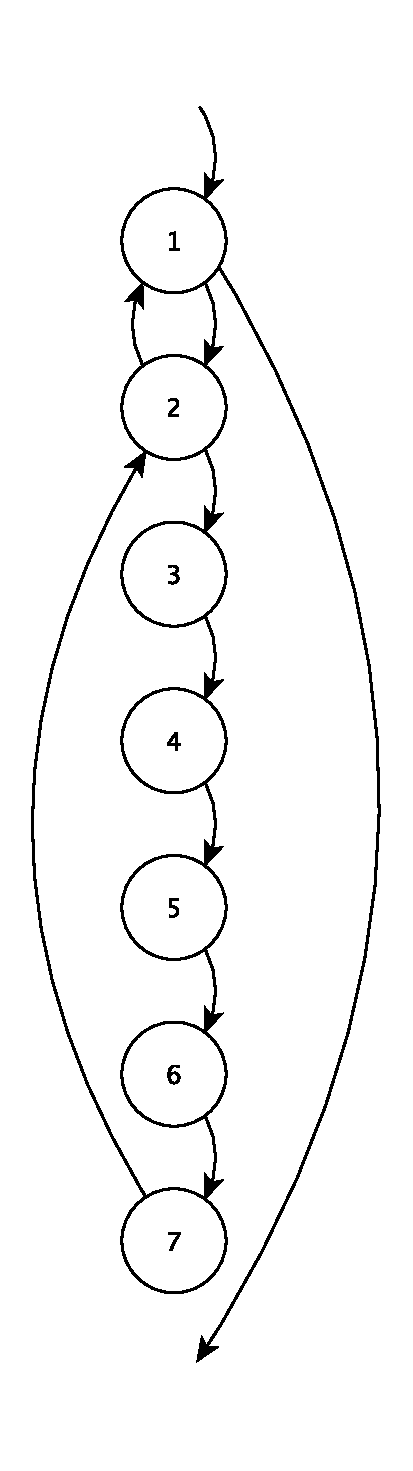
\includegraphics[width=0.32\linewidth]{../og.pdf}
    \captionof{figure}{Граф управления}
    \label{img:graph1}
  \end{tabular}
\end{table}

\begin{table}[h!]
  \centering
  \begin{tabular}{p{1\linewidth}}
    \centering
    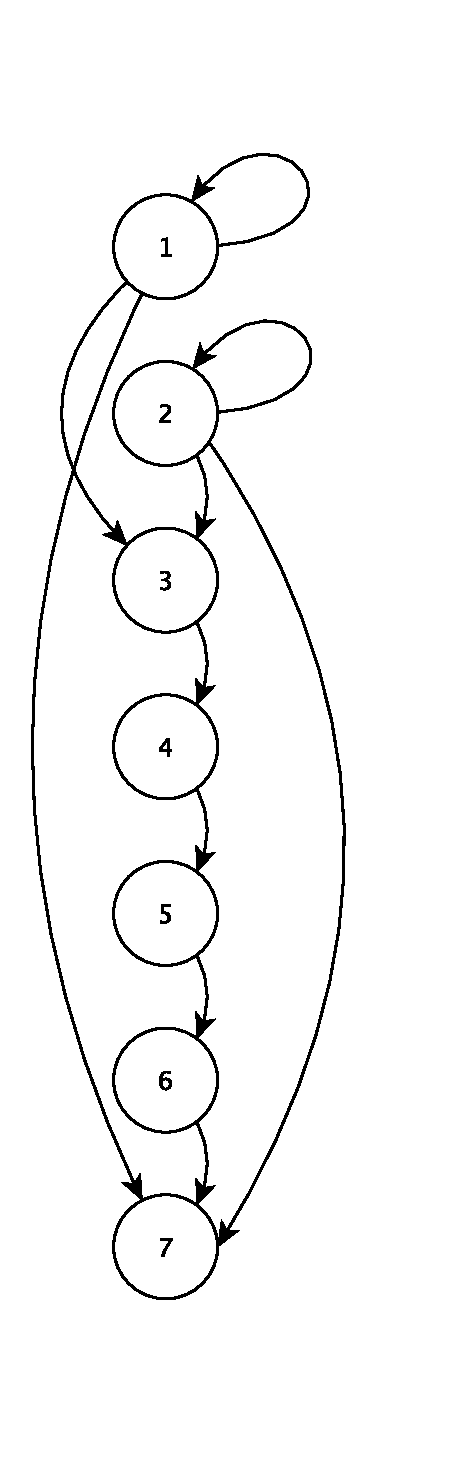
\includegraphics[width=0.4\linewidth]{../ig.pdf}
    \captionof{figure}{Информационный граф}
    \label{img:graph2}
  \end{tabular}
\end{table}

\begin{table}[h!]
  \centering
  \begin{tabular}{p{1\linewidth}}
    \centering
    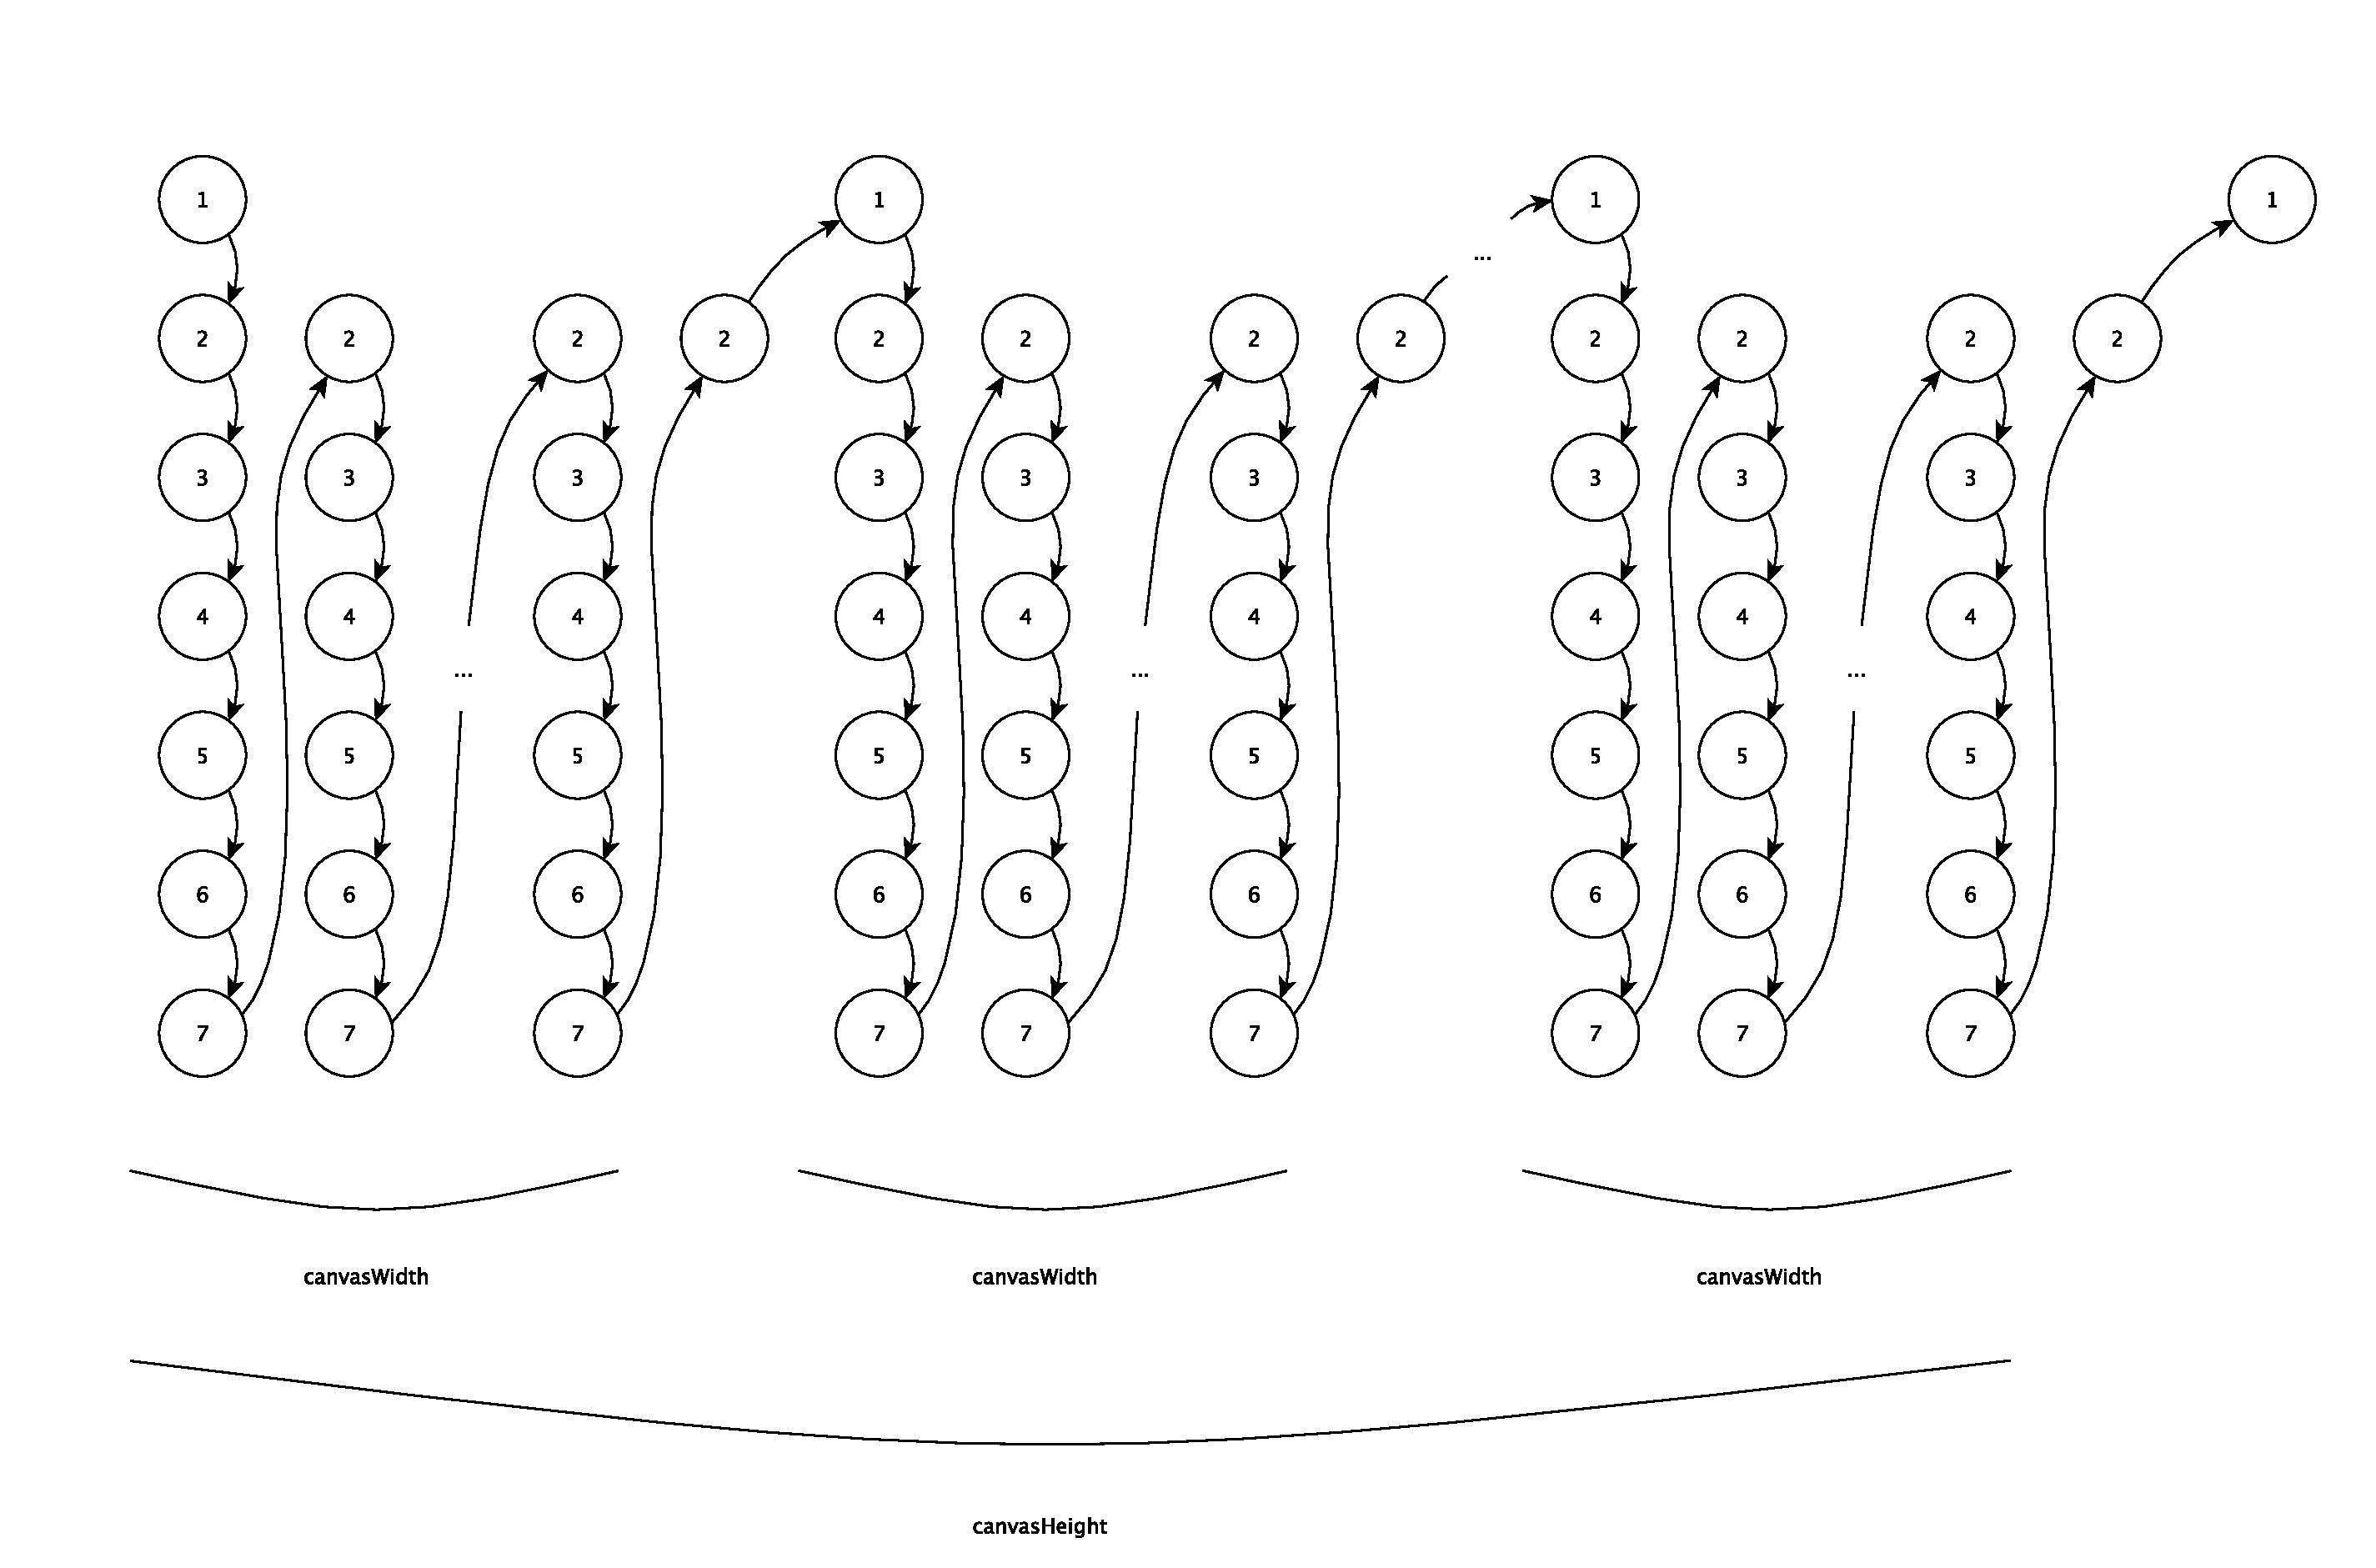
\includegraphics[width=0.9\linewidth]{../oh.pdf}
    \captionof{figure}{Операционная история}
    \label{img:graph3}
  \end{tabular}
\end{table}

\begin{table}[h!]
  \centering
  \begin{tabular}{p{1\linewidth}}
    \centering
    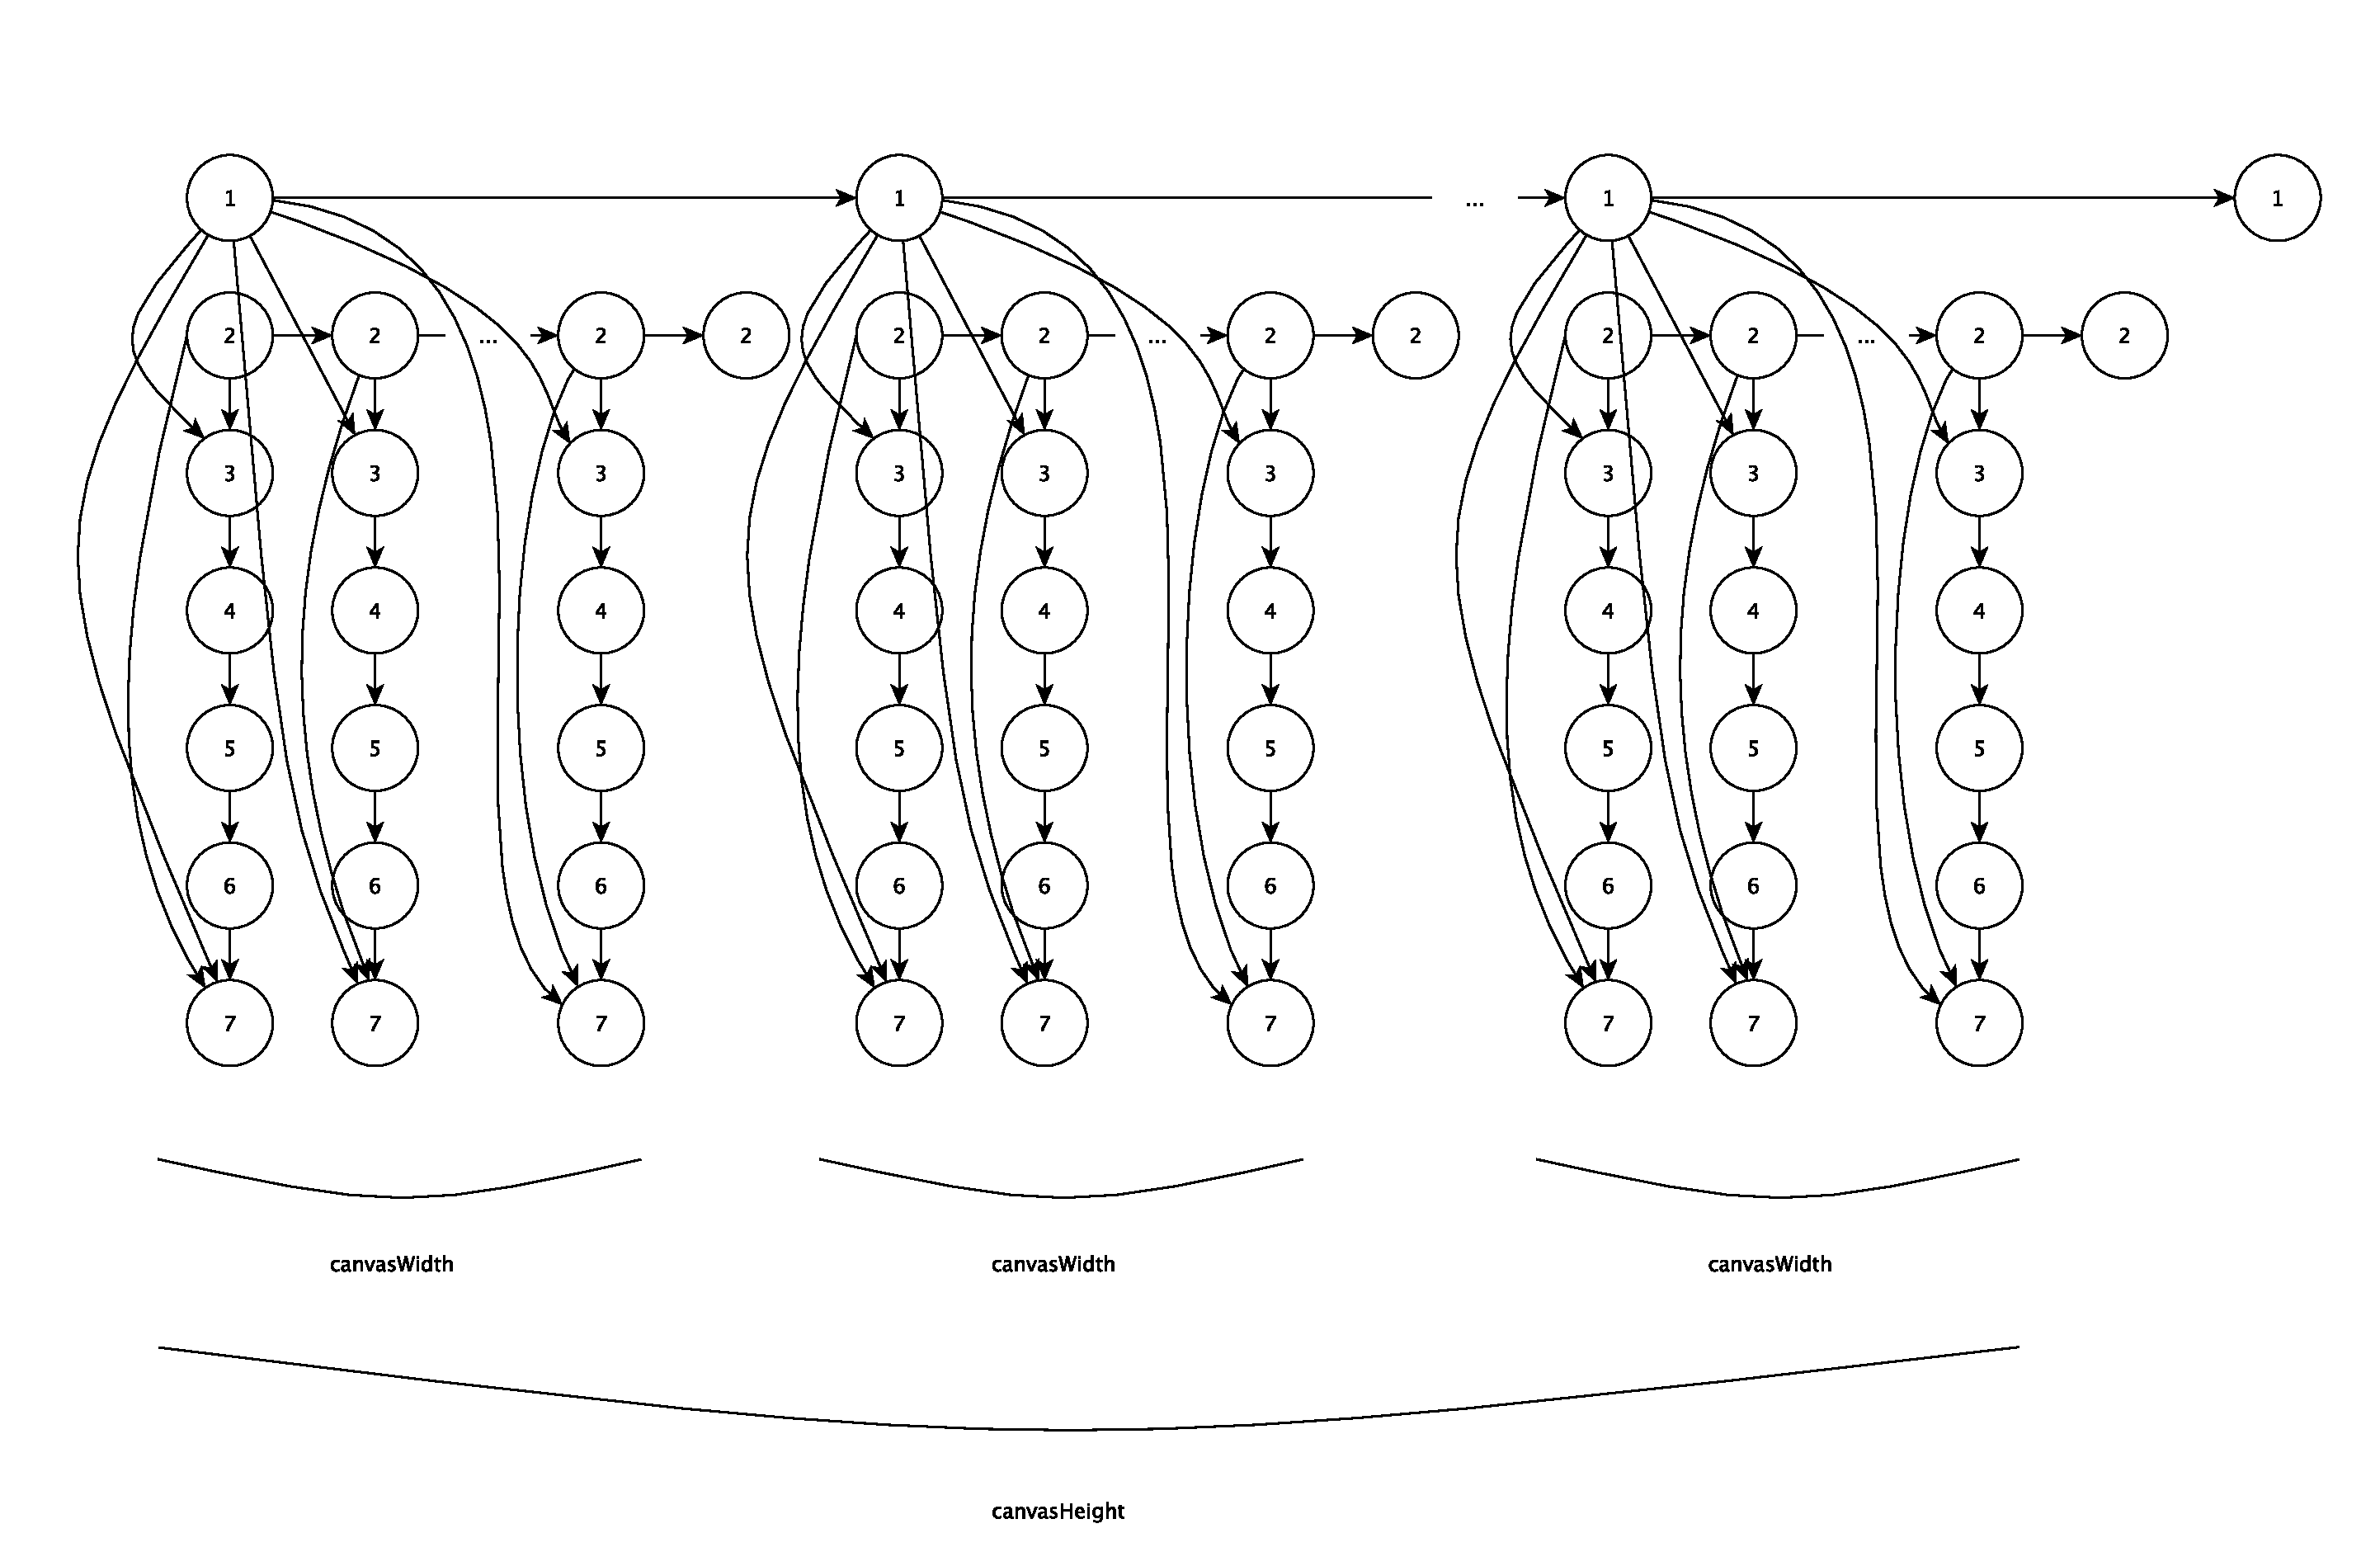
\includegraphics[width=0.9\linewidth]{../ih.pdf}
    \captionof{figure}{Информационная история}
    \label{img:graph4}
  \end{tabular}
\end{table}

\newpage